\hypertarget{sh__move_8c}{
\section{sh\_\-move.c File Reference}
\label{sh__move_8c}\index{sh_move.c@{sh\_\-move.c}}
}


\subsection{Detailed Description}
\begin{Desc}
\item[For internal use only.]
This file contains the implementation of the \hyperlink{group__dbprim__smat_ga21}{sh\_\-move()} function, used to move sparse matrix entries from one place to another in a sparse matrix head list.\end{Desc}


Definition in file \hyperlink{sh__move_8c-source}{sh\_\-move.c}.

{\tt \#include \char`\"{}dbprim.h\char`\"{}}\par
{\tt \#include \char`\"{}dbprim\_\-int.h\char`\"{}}\par


Include dependency graph for sh\_\-move.c:\begin{figure}[H]
\begin{center}
\leavevmode
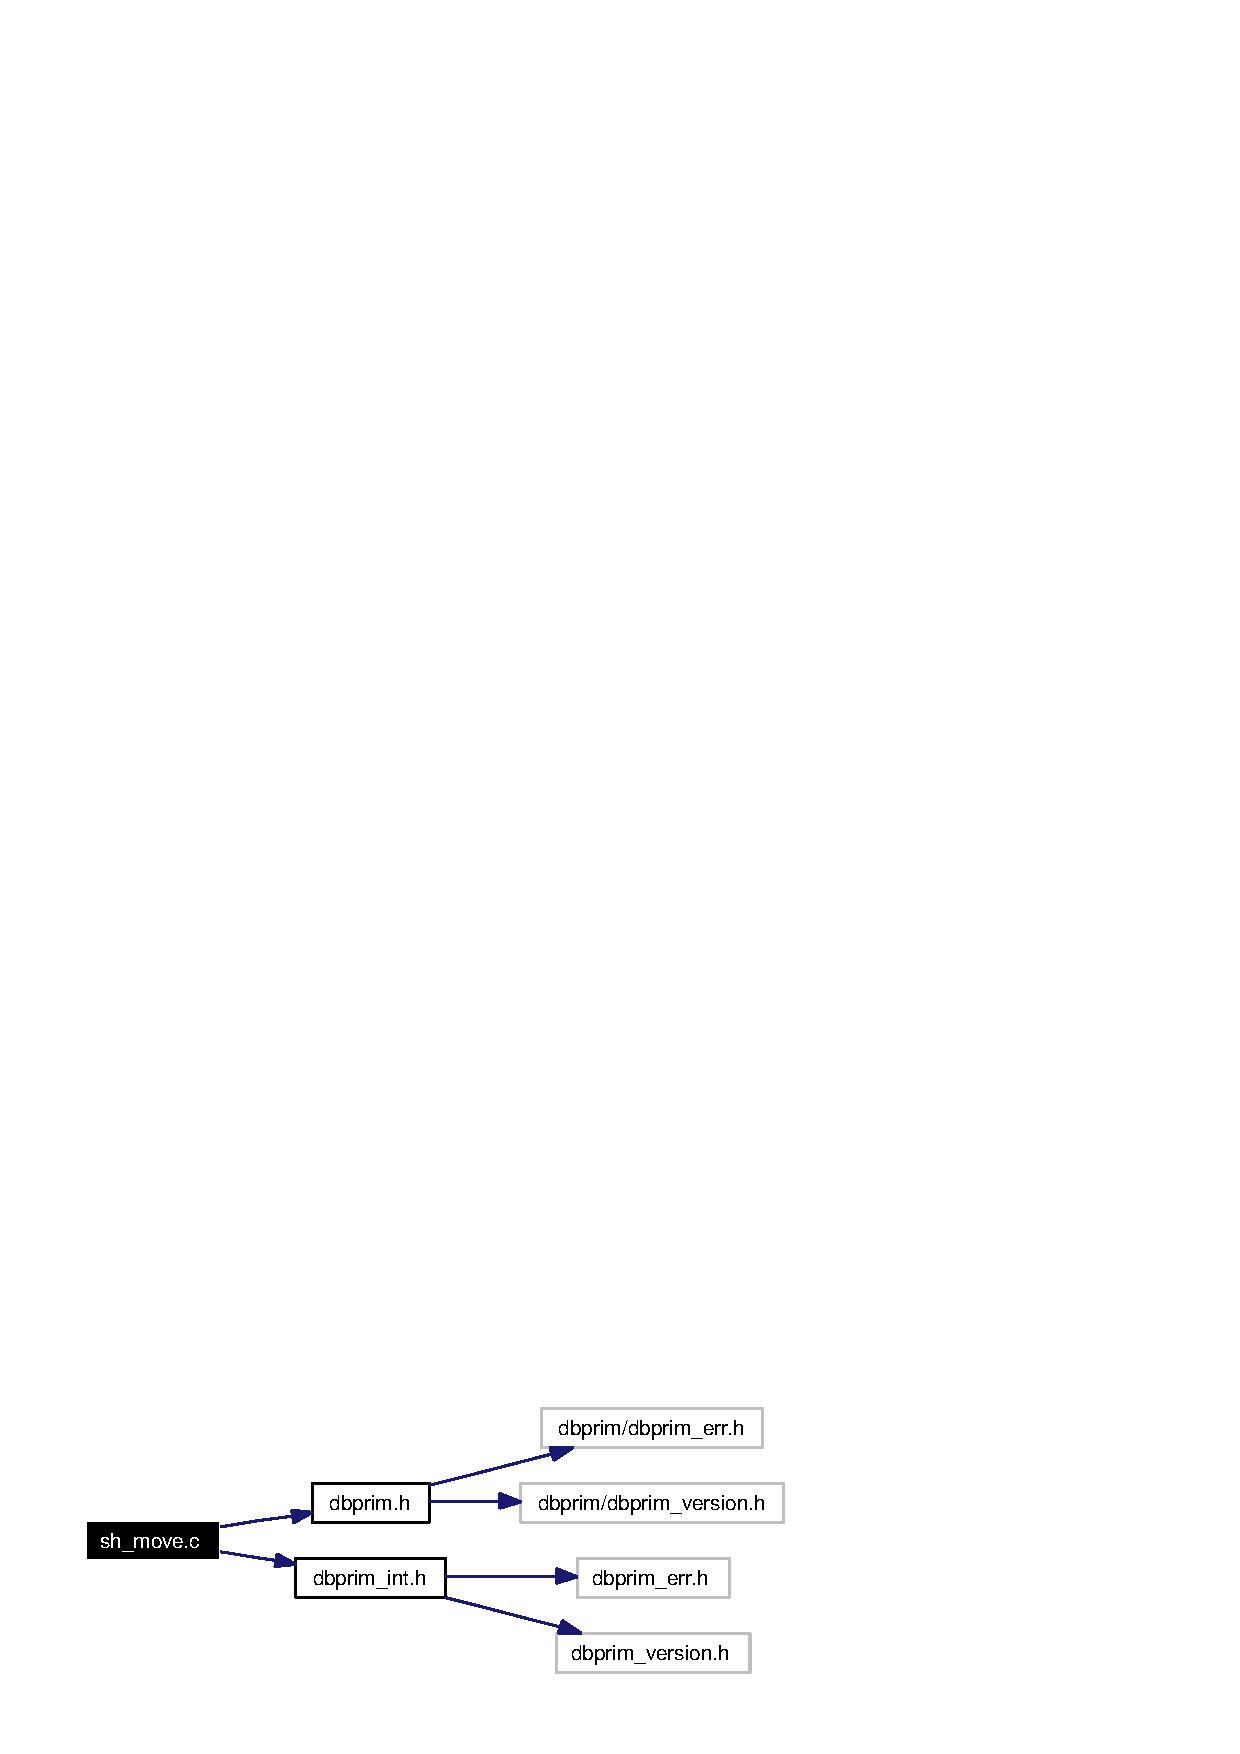
\includegraphics[width=190pt]{sh__move_8c__incl}
\end{center}
\end{figure}
\subsection*{Functions}
\begin{CompactItemize}
\item 
unsigned long \hyperlink{group__dbprim__smat_ga21}{sh\_\-move} (\hyperlink{struct__smat__head__s}{smat\_\-head\_\-t} $\ast$head, \hyperlink{struct__smat__entry__s}{smat\_\-entry\_\-t} $\ast$elem, \hyperlink{group__dbprim__link_ga4}{link\_\-loc\_\-t} loc, \hyperlink{struct__smat__entry__s}{smat\_\-entry\_\-t} $\ast$elem2)
\begin{CompactList}\small\item\em Move an entry within a row or column list. \item\end{CompactList}\end{CompactItemize}
